\fakesection{Simuleren van Sparen en Beleggen}

\begin{center}
\textit{De broncode bevindt zich in de \texttt{src} folder. Het algemene script (\texttt{src/s0216676\_script}) is opgedeeld in secties, \'e\'en per opgave. Elke opgave wordt hieronder afzonderlijk beantwoord. Aan het einde van elk antwoord wordt (indien nodig) de broncode weergegeven.}
\end{center}

%%%
%%%
%%%

\fakesubsection{Opdracht 1}

Hier is een implementatie :

\begin{lstlisting}
function [yield, invested, value] = s0216676_simulateSavingInvesting(budget, rate, months)
    value = repelem(budget * 1.02 .^ (0:floor(months/12)), 1, 12); 
    invested = sum(value(1:months));
    for j = 13:12:months % Consider each month of january
    	win = sum(value(j-12:j-1) .* (((12:-1:1)/12) * (rate/100))); % Calculate savings
    	value(j) = value(j) + (win - 0.15 * (win > 980) * (win - 980));
        value(j-12:j) = cumsum(value(j-12:j)); % Accumulate sums
    end
    value = value(1:months); value(j:end) = cumsum(value(j:end));
    yield = value(months) / invested - 1;
end
\end{lstlisting}

%%%
%%%
%%%

\fakesubsection{Opdracht 2}

Het resultaat van de gegeven code is te zien in figuur \ref{fig:op2}. De totale investering bedraagt zo'n 96091 euro. De relatieve winsten bedragen 5.46\%, 11.34\%, 23.34\% en 50.82\%.

\vspace{0.3cm}
\begin{figure}[h]
\centering
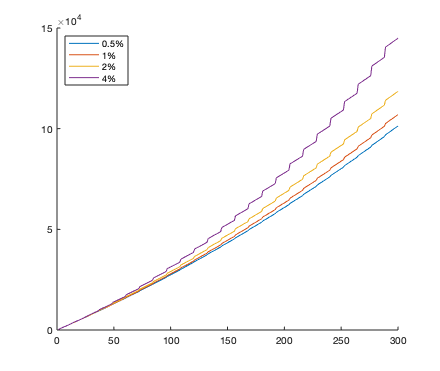
\includegraphics[width=0.45\textwidth]{res/op2.png}
\caption{Simulatie van spaarrekeningen met verschillende rentevoeten.}
\label{fig:op2}
\end{figure}

%%%
%%%
%%%

\fakesubsection{Opdracht 3}

Het bestand wordt ingeladen.

\begin{lstlisting}
load('Funds.mat')
\end{lstlisting}

%%%
%%%
%%%

\fakesubsection{Opdracht 4}

Men kan de parameters berekenen door eerst $\sigma$ te bepalen op basis van de rendementen, het gemiddelde te berekenen van diezelfde rendementen en vervolgens $\mu$ daaruit te bepalen.\\
\par\noindent De bekomen parameters bedragen $\mu = 3.208565\times 10^{-3}, \sigma = 3.070426\times 10^{-2}$ (voor \texttt{EUN5}) en $\mu = 7.857782\times 10^{-3}, \sigma = 3.277546\times 10^{-2}$ (voor \texttt{VWRL}).

\begin{lstlisting}
function [mu,sigma] = s0216676_estimateParameters(s)
    rendements = log(s(2:end) ./ s(1:end-1));q
    sigma = std(rendements);
    mu = mean(rendements) + 0.5 * sigma^2;
end
\end{lstlisting}

%%%
%%%
%%%

\fakesubsection{Opdracht 5}

De implementatie maakt gebruik van een eenvoudige \mcode{for} loop.

\begin{lstlisting}
function [path] = s0216676_simulateFundPath(initialPrice, mu, sigma, months)
    alpha = mu - 0.5 * sigma^2;
    path = [initialPrice 2:months];
    for t = 2:months
        path(t) = path(t-1) * exp(alpha + sigma * randn);
    end
end
\end{lstlisting}

%%%
%%%
%%%

\fakesubsection{Opdracht 6}

In figuur \ref{fig:op6} worden de resulterende paden afgebeeld. Een aantal paden wijken af van de werkelijke koers afgebeeld in de opgave, maar de meesten komen ruwweg overeen. De initi\"ele waarde bedraagt telkens 74.19 euro wat overeenstemt met de waarde in dollar op 26 november 2019.

\begin{figure}[h]
\centering
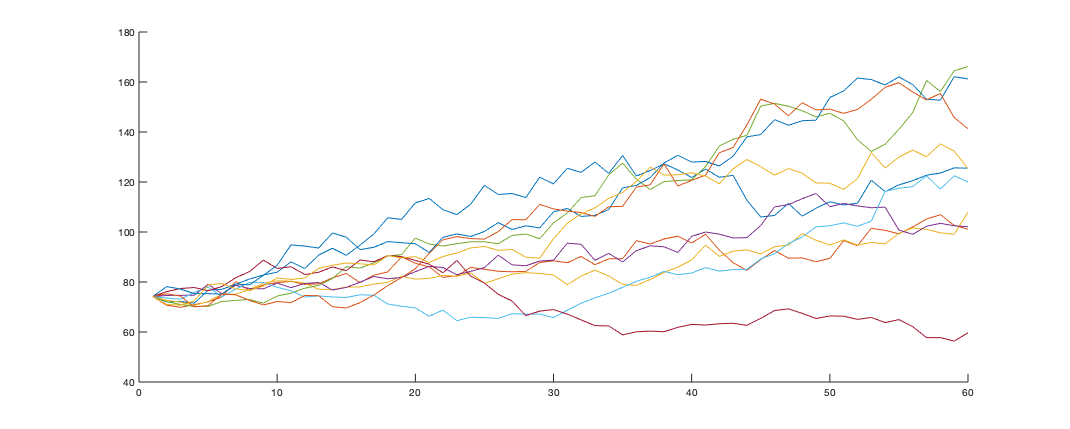
\includegraphics[width=\textwidth]{res/op6.png}
\caption{Simulatie van spaarrekeningen met verschillende rentevoeten.}
\label{fig:op6}
\end{figure}

\begin{lstlisting}
figure; hold all;
for i = 1:10
    plot(s0216676_simulateFundPath(74.19, mu, sigma, 60)); % Converted to euros (26/11/2019)
end
\end{lstlisting}

%%%
%%%
%%%

\fakesubsection{Opdracht 7}

De cumulatieve distributiefuncties zijn afgebeeld in figuur \ref{fig:op7}. Op basis hiervan kan men met een zekere graad van vertrouwen beweren dat de log-rendementen effectief normaal verdeeld is. Normaal gezien maakt men gebruik van specifieke testen om dit te kwantificeren.

\begin{figure}[h]
\centering
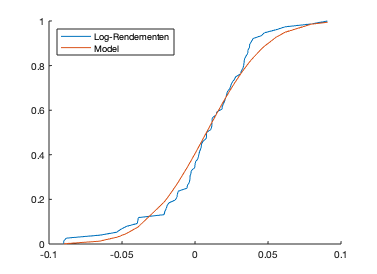
\includegraphics[width=0.5\textwidth]{res/op7.png}
\caption{Cumulatieve distributiefuncties van de log-rendementen en het model.}
\label{fig:op7}
\end{figure}

\begin{lstlisting}
[f,x] = ecdf(log(VWRL(2:end) ./ VWRL(1:end-1)));
[f_norm] = normcdf(x, mu, sigma);
figure; hold all;
plot(x, f, x,f_norm);
legend('Log-Rendementen', 'Model', 'Location', 'NorthWest');
\end{lstlisting}

%%%
%%%
%%%

\fakesubsection{Opdracht 8}

Het kon ook met een lus, maar ik deed het deze keer met ingebouwde functies. 

\begin{lstlisting}
function [yield, invested, value, units] = s0216676_simulateFundInvestingPath(budget,pricePath,alpha)
    months = size(alpha,1);
    budgets = repelem(budget * (1.02 .^ (0:floor(months/12))'), 12, 2);
    invested = sum(budgets(1:months,1));
    units = (budgets(1:months,:) .* [alpha (1-alpha)] - 6) / 1.0035;
    for i = 1:2
        units(units(:,i) < 0, 3-i) = (budgets(units(:,i) < 0) - 6) / 1.0035;
        units(units(:,i) < 0, i) = 0;
    end
    units = cumsum(units ./ pricePath);
    value = units .* pricePath;
    yield = sum(value(end,:)) / invested - 1;
end
\end{lstlisting}

%%%
%%%
%%%

\fakesubsection{Opdracht 9}

De resulterende figuren zijn afgebeeld op de volgende pagina.

\newgeometry{top=1.5cm,bottom=1.5cm}
\thispagestyle{empty}

\topskip0pt
\vspace*{\fill}

\begin{figure}[h]
\centering
\subfloat[Iteratie 1]{{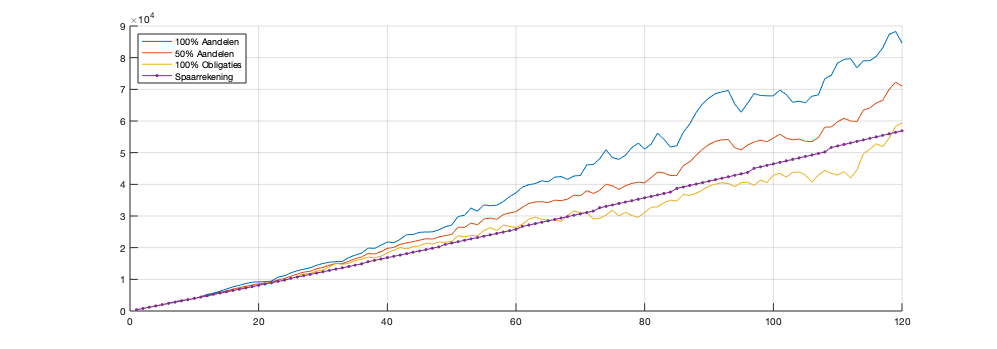
\includegraphics[width=\textwidth]{res/op8a.png} }}\\
\subfloat[Iteratie 2]{{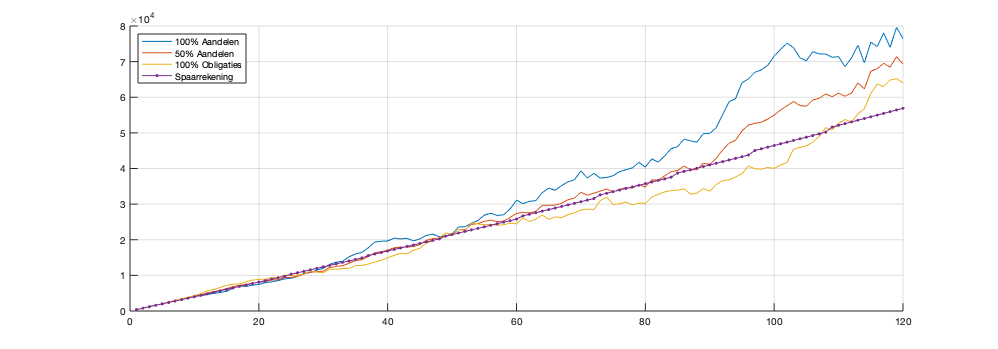
\includegraphics[width=\textwidth]{res/op8b.png} }}
\caption{Waarde van vier type investeringen doorheen een periode van 120 maanden.}%
\label{fig:op8}
\end{figure}

\begin{figure}[h]
\centering
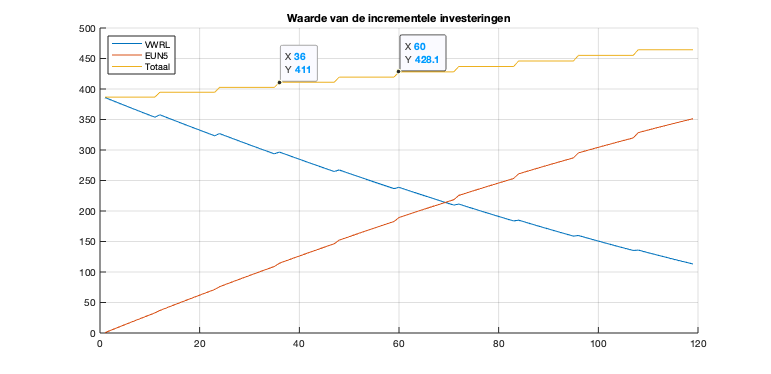
\includegraphics[width=0.95\textwidth]{res/op9b.png}
\caption{Waarde van de investering op maandelijkse basis.}
\label{fig:op9a}
\end{figure}

\vspace*{\fill}

\restoregeometry

%%%
%%%
%%%

\fakesubsection{Opdracht 10}

De functie werd als volgt ge\"implementeerd.

\begin{lstlisting}
function [yields,invested] = s0216676_simulateFundInvesting(budget, priceHistory, alpha, N)
    months = size(alpha, 2);
    [mu1,sigma1] = s0216676_estimateParameters(priceHistory(:,1));
    [mu2,sigma2] = s0216676_estimateParameters(priceHistory(:,2));
    yields = 1:N;
    for i = 1:N
        path1 = s0216676_simulateFundPath(priceHistory(end,1), mu1, sigma1, months);
        path2 = s0216676_simulateFundPath(priceHistory(end,2), mu2, sigma2, months);
        [yields(i),invested,~,~] = s0216676_simulateFundInvestingPath(budget, [path1 path2], alpha);
    end
end
\end{lstlisting}

%%%
%%%
%%%

\fakesubsection{Opdracht 11}

De histogrammen staan gezamenlijk afgebeeld in figuur \ref{fig:op11} (zie volgende bladzijde) en afzonderlijk hieronder. Het rendement van de spaarrekening bedroeg ongeveer 47.22\%. Het valt op dat hoe agressiever men speelt, hoe waarschijnlijker het wordt dat men grote winsten maakt.

\begin{figure}[h]
\centering
\subfloat[Agressief]{{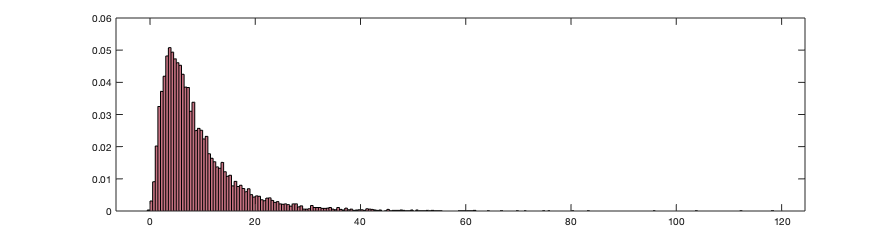
\includegraphics[width=0.9\textwidth]{res/op11a.png} }}\\
\subfloat[Gebalanceerd]{{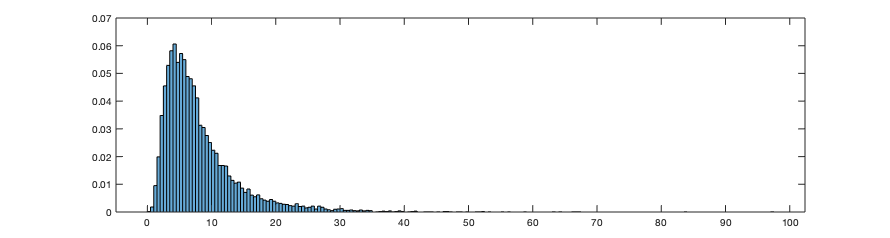
\includegraphics[width=0.9\textwidth]{res/op11b.png} }}\\
\subfloat[Defensief]{{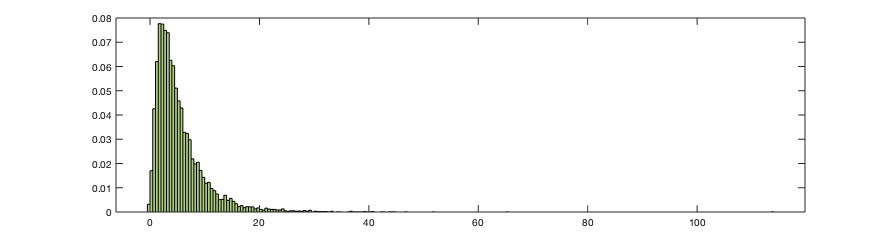
\includegraphics[width=0.9\textwidth]{res/op11c.png} }}
\caption{Afzonderlijke histogrammen gegenereerd na Monte-Carlo simulaties.}%
\label{fig:op11sep}
\end{figure}

\newgeometry{top=1.5cm,bottom=1.5cm}
\begin{sidewaysfigure}[h]
\centering
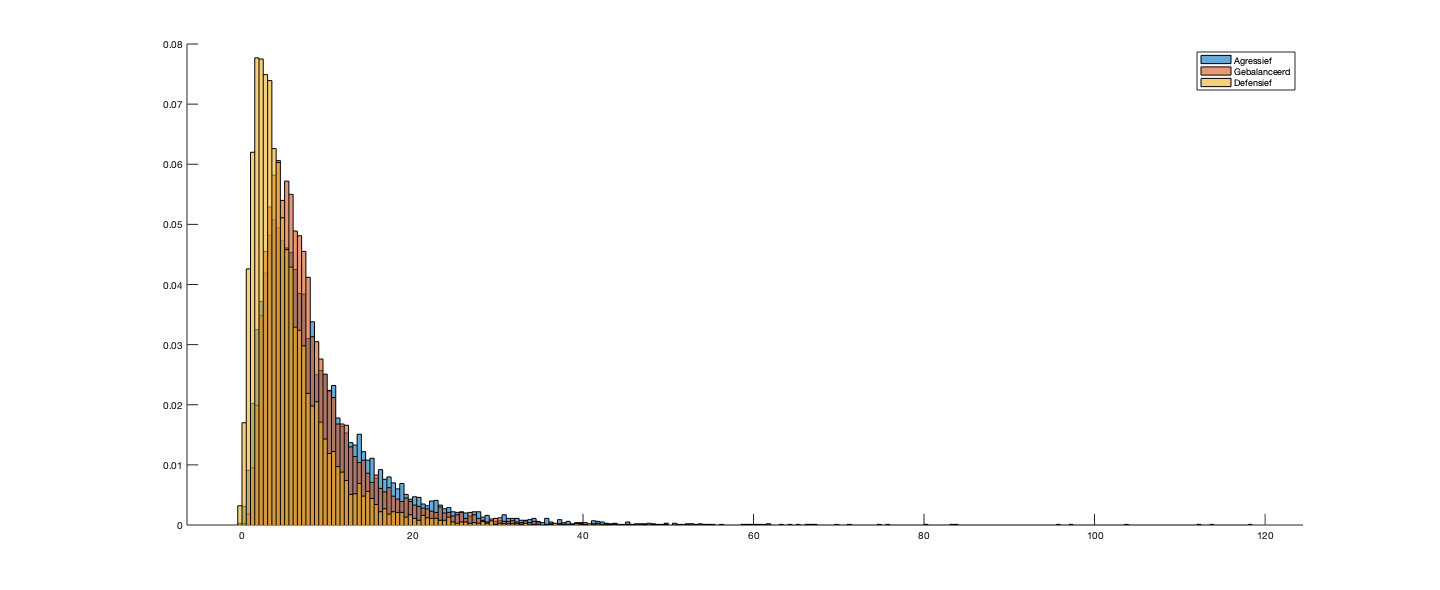
\includegraphics[width=0.95\textwidth]{res/op11.png}
\caption{Histogram gegenereerd na het uitvoeren van de Monte-Carlo simulaties.}
\label{fig:op11}
\end{sidewaysfigure}
\thispagestyle{empty}
\restoregeometry

%%%
%%%
%%%

\fakesubsection{Opdracht 12}

In tabellen \ref{tab:op12a} en \ref{tab:op12b} worden eerst de kwantielen beschouwd (met $x=28, y=76$), vervolgens de kans op negatieve eindrendementen en ten slotte de kans op het behalen van een vermogen van 750.000 euro. Het mediaan van het vermogen bereikt op de leeftijd van 70 jaar bedroeg X, Y, Z en W euro voor de vier scenario's. Enkel XYZ zou tot het gewenste maandelijkse inkomen van 1790 euro leiden.

\begin{table}[h]
\centering
\begin{tabular}{cc|cccccc}
\multicolumn{1}{l}{}                       &               & 0.1\%     & 2.5\%     & 25\%      & 50\%      & 75\%      & 97.5\%    \\ \hline
\multirow{4}{*}{\textit{n = 300}}          & Spaarrekening & \textit{} & \textit{} & \textit{} & \textit{} & \textit{} & \textit{} \\
                                           & Agressief    & \textit{} & \textit{} & \textit{} & \textit{} & \textit{} & \textit{} \\
                                           & Gebalanceerd  & \textit{} & \textit{} & \textit{} & \textit{} & \textit{} & \textit{} \\
                                           & Defensief     & \textit{} & \textit{} & \textit{} & \textit{} & \textit{} & \textit{} \\ \hline
\multirow{4}{*}{\textit{n = 12 *(70 - x)}} & Spaarrekening & \textit{} & \textit{} & \textit{} & \textit{} & \textit{} & \textit{} \\
                                           & Aggressive    & \textit{} & \textit{} & \textit{} & \textit{} & \textit{} & \textit{} \\
                                           & Gebalanceerd  & \textit{} & \textit{} & \textit{} & \textit{} & \textit{} & \textit{} \\
                                           & Defensief     & \textit{} & \textit{} & \textit{} & \textit{} & \textit{} & \textit{}
\end{tabular}
\caption{Kwantielen voor de 8 mogelijke scenario's.}
\label{tab:op12a}
\end{table}

\begin{table}[h]
\centering
\begin{tabular}{cc|c|c}
\multicolumn{1}{l}{}                       &               & $P(y<0)$     & $P(v\geq 750.000)$      \\ \hline
\multirow{4}{*}{\textit{n = 300}}          & Spaarrekening & \textit{} & \textit{}  \\
                                           & Agressief    & \textit{} & \textit{} \\
                                           & Gebalanceerd  & \textit{} & \textit{} \\
                                           & Defensief     & \textit{} & \textit{}  \\ \hline
\multirow{4}{*}{\textit{n = 12 *(70 - x)}} & Spaarrekening & \textit{} & \textit{}  \\
                                           & Aggressive    & \textit{} & \textit{}  \\
                                           & Gebalanceerd  & \textit{} & \textit{} \\
                                           & Defensief     & \textit{} & \textit{} 
\end{tabular}
\caption{Kans op negatieve eindrendementen en op het bereiken van een vermogen van 750.000 euro voor de 8 mogelijke scenario's.}
\label{tab:op12b}
\end{table}
